\documentclass[12pt]{article}

\usepackage[a4paper,left=3cm,right=1cm,top=15mm,bottom=2cm,bindingoffset=0cm]{geometry}
\usepackage{amsmath,amsthm,amssymb}
\usepackage{graphicx}
\usepackage{mathtext}
\usepackage{listings}
\usepackage{color}
\usepackage{caption}
\usepackage{hyperref}
\usepackage[T1,T2A]{fontenc}
\usepackage[utf8]{inputenc}
\usepackage[english,russian]{babel}
\usepackage{multirow}
\graphicspath{{img/}}
\DeclareGraphicsExtensions{.pdf,.png,.jpg}
\DeclareCaptionFont{white}{\color{white}} 
\DeclareCaptionFormat{listing}{\colorbox{gray}{\parbox{\textwidth}{#1#2#3}}}
\captionsetup[lstlisting]{format=listing,labelfont=white,textfont=white}
\newcommand{\specialcell}[2][c]{%
  \begin{tabular}[#1]{@{}c@{}}#2\end{tabular}}
\begin{document}

\begin{titlepage}
\begin{center}
Министерство науки и высшего образования Российской Федерации\\
Федеральное государственное бюджетное образовательное учреждение высшего образования\\
ИРКУТСКИЙ НАЦИОНАЛЬНЫЙ ИССЛЕДОВАТЕЛЬСКИЙ ТЕХНИЧЕСКИЙ УНИВЕРСИТЕТ\\
Институт информационных технологий и анализа данных\\
\vspace{7cm}
\large ОТЧЕТ\\
По лабораторной работе по дисциплине\\
\underline{Основы теории управления}\\
\underline{Лабораторная работа №5}\\
\underline{<<Исследование автоматической системы с запаздыванием>>}\\
Вариант 22
\end{center}
\vspace{9cm}
\begin{flushright}
Выполнил \\
Студент группы АСУб 18-1 \\
Вдовиченко В.А. \\
\end{flushright}
\begin{flushright}
Проверила:\\
Серышева И.А. \\
\end{flushright}
\end{titlepage}
\section{Заданная структурная схема автоматической системы с заданными значениями параметров}
\textbf{Цель работы: } ознакомление с автоматическими системами с запаздыванием; моделирование звена запаздывания; устойчивость автоматических систем с запаздыванием; влияние запаздывание на качество переходных процессов. \\
\begin{figure}[h]
    \label{graphs}
     \centering
    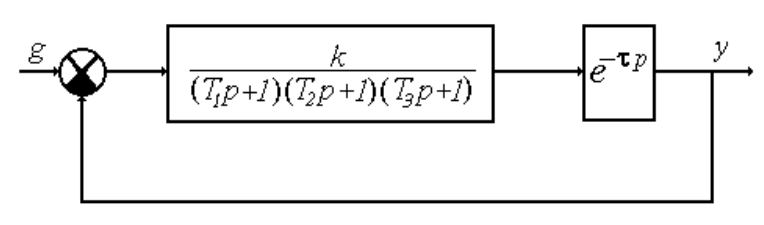
\includegraphics[width = 12cm]{структурная схема.png}
    \caption{Структурная схема исследуемой автоматической системы}
\end{figure}
 
Значения параметров звена: \\
$k = 150$\\
$T_1 =25$\\
$T_2 = 0.1$ \\
$T_3 = 0.01$

Звено охватывается единичной отрицательной обратной связью. \\ 

\section{Описание процесса построения АФЧХ для заданной автоматической
системы.}
Передаточная функция разомкнутой системы с запаздыванием:
\begin{equation}
    W_{р}(p) = W_1(p)W_{зап}(p) = \frac{k}{(T_1p + 1)(T_2p + 1)(T_3p + 1)}e^{-\tau p} 
\end{equation}
Запаздывающее звено находится в прямой цепи, поэтому передаточная функция замкнутой системы равна 
\begin{equation}
    W_{зам}(p) = \frac{W_{р}(p)}{1 + W_{р}(p)} = \frac{\frac{ke^{-\tau p}}{(T1p + 1)(T_2p + 1)(T_3p + 1))}}{\frac{(T_1p + 1)(T_2p + 1)(T_3p + 1) + ke^{-\tau p}}{(T_1p + 1)(T_2p + 1)(T_3p + 1)}} = \frac{ke^{-\tau p}}{(T_1p + 1)(T_2p + 1)(T_3p + 1) + ke^{-\tau p}}
\end{equation}
Характеристическое уравнение:
\begin{equation}
    (T_1p + 1)(T_2p + 1)(T_3p + 1) + ke^{-\tau p} = 0
\end{equation}
Нахождение корней характеристического уравнения затруднительно, поэтому для исследования устойчивости системы с запаздыванием будем использовать критерий устойчивости Найквиста. \\
Найдём устойчивость предельной системы (при $\tau = 0$) в разомкнутом состоянии.
\begin{equation}
    W_{пред}(p) = \frac{k}{(T_1p + 1)(T_2p + 1)(T_3p + 1)}
\end{equation}
Характеристическое уравнение предельной системы:
\begin{equation}
\begin{gathered}
    (T_1p + 1)(T_2p + 1)(T_3p + 1) = 0 \\
    \left[
       \begin{gathered}
        p_1 = -\frac{1}{T_1}, \\
        p_2 = -\frac{1}{T_2}, \\
        p_3 = -\frac{1}{T_3}.
     \end{gathered}
     \right.
\end{gathered}
\end{equation}
Все корни характеристического уравнения отрицательны, значит предельная система в разомкнутом состоянии устойчива. В данном случае для устойчивости замкнутой системы необходимо и достаточно, чтобы АФЧХ разомкнутой системы при изменении $\omega$ от 0 до $\infty$ не охватывала точку с координатами $[-1, j0]$. \\
Подставим в передаточную функцию разомкнутой системы чисто мнимое значение $p = j\omega$. Алгебраическая форма: 
\begin{equation}
    W_р(p) = \frac{k}{(T_1j\omega + 1)(T_2j\omega + 1)(T_3j\omega + 1)}e^{-\tau j\omega} = (Re(\omega) + jIm(\omega))e^{-\tau j\omega}
\end{equation}
Показательная форма: 
\begin{equation}
    W_р(p) = A(\omega)e^{j\phi(\omega)}e^{-\tau j\omega} = A(\omega)e^{j(\phi(\omega)-\tau \omega)} 
\end{equation}
Где: 
\begin{equation}
    \begin{gathered}
        A(\omega) = \sqrt{Re^2(\omega) + Im^2(\omega)}\\
        \phi(\omega) =\arctan{\frac{Im(\omega)}{Re(\omega)}} 
    \end{gathered}
\end{equation}
Звено запаздывания не меняет модуля $A(\omega)$ АФЧХ разомкнутой системы, а вносит лишь дополнительный отрицательный фазовый сдвиг, пропорциональный частоте, причем коэффициентом пропорциональности является время запаздывания $\tau$. \\
Чтобы найти амплитуду и фазу предельной системы, представим звено в виде 3х последовательных апериодических звеньев первого порядка. 
\begin{equation}
    \begin{gathered}
    W_{пред}(j\omega) = W_1(j\omega)W_2(j\omega)W_3(j\omega) = \frac{k}{T_1j\omega + 1}*\frac{1}{T_2j\omega + 1}*\frac{1}{T_3j\omega + 1} \\
    A(\omega) = A_1(\omega)A_2(\omega) \\
    \phi(\omega) = \phi_1(\omega) + \phi_2(\omega)
    \end{gathered}
\end{equation}
Амплитуда и фаза 1-го звена: 
\begin{equation}
    \begin{gathered}
    A_1(\omega) = \frac{k}{\sqrt{1 + T_1^2\omega^2}} \\
    \phi_1(\omega) = -\arctan{T_1\omega}
    \end{gathered}
\end{equation}
Амплитуда и фаза 2-го и 3-го звена:
\begin{equation}
    \begin{gathered}
     A_{2,3}(\omega) = \frac{1}{\sqrt{1 + T_{2,3}^2\omega^2}} \\
    \phi_{2,3}(\omega) = - \arctan{T_{2,3}\omega} 
    \end{gathered}
\end{equation}
Результирующие амплитуда и фаза: 
\begin{equation}
    \begin{gathered}
        A(\omega) = \frac{k}{\sqrt{(1 + T_1^2\omega^2)(1 + T_2^2\omega^2)(1 + T_3^2\omega^2)}} \\
        \phi(\omega) = -\arctan{T_1\omega} - \arctan{T_2\omega} - \arctan{T_3\omega} 
    \end{gathered}
\end{equation}
\begin{equation}
    \begin{cases}
        Re(\omega) = A(\omega)\cos{\phi(\omega)} \\
        Im(\omega) = A(\omega)\sin{\phi(\omega)} 
    \end{cases}
\end{equation}

\begin{figure}[h!]
     \centering
    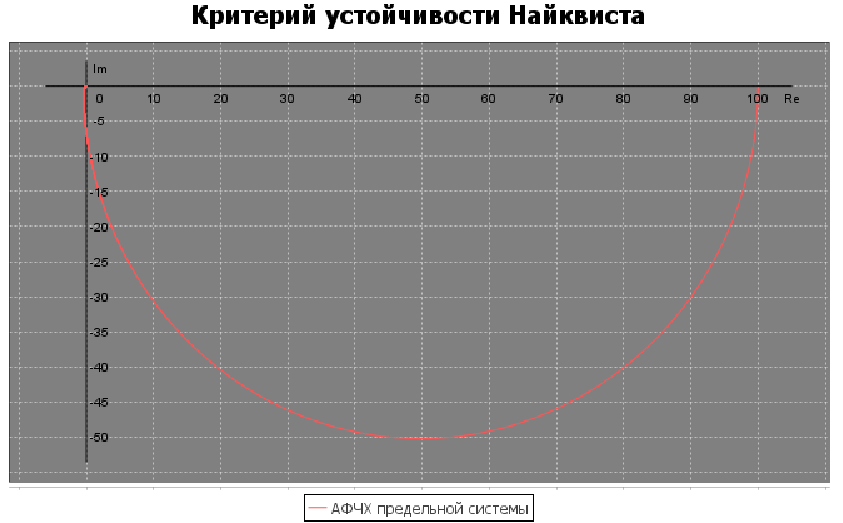
\includegraphics[width = \linewidth]{АФЧХ.png}
    \caption{АФЧХ}
\end{figure} 
График не охватывает точку с координатами $[-1, j0]$, значит система устойчива. 
\newpage
\section{Описание процесса определения $\tau_{кр}$ графическим способом}
\begin{figure}[h]
     \centering
    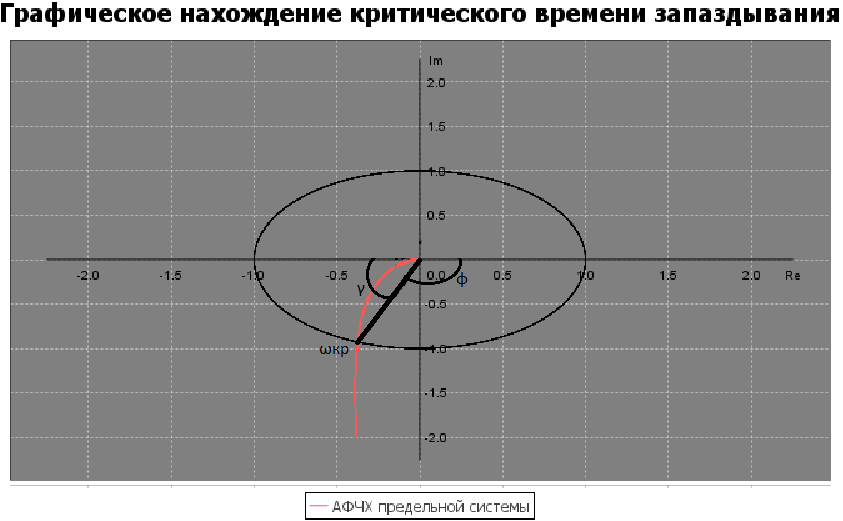
\includegraphics[width = \linewidth]{графически.png}
    \caption{Определение $\tau_{кр}$ графическим способом}
\end{figure} 
Чтобы определить $\tau_{кр}$ графически, построим окружность единичного радиуса. Точка пересечения годографа $W(j\omega)$ с этой окружностью определяет частоту $\omega_{кр}$. Время запаздывания $\tau_{кр}$ определяется по формуле
\begin{equation}
    \tau_{кр} = \frac{\pi - \phi_{кр}}{\omega_{кр}} = \frac{\gamma_{кр}}{\omega_{кр}}
\end{equation}
Значения, вычисленные по графику: 
\begin{equation}
    \begin{gathered}
    \omega_{кр} = 5.295 \\
    \phi_{кр} = -2.1031109 \\
    \tau_{кр} = 0.19582418
    \end{gathered}
\end{equation}
\newpage
\section{Аналитические выражения, с помощью
которых определено значение  $\tau_{кр}$}
Значения $\tau_{кр}$ и $\omega_{кр}$ определяются из уравнения 
\begin{equation}
    W_р(j\omega_{кр}) = W_1(j\omega_{кр})W_{зап}(j\omega_{кр}) = 1 
\end{equation}
Которое можно представить двумя уравнениями: 
\begin{equation}
    \begin{cases}
    A(\omega_{кр}) = 1, \\
    \phi(\omega_{крит}) = \phi_1(\omega_{крит}) - \tau_{кр}\omega_{крит}
    \end{cases}
\end{equation}
Приравняем амплитуду к 1:
\begin{equation}
\begin{gathered}
      A(\omega_{кр}) = \frac{k}{\sqrt{(1 + T_1^2\omega_{кр}^2)(1 + T_2^2\omega_{кр}^2)(1 + T_3^2\omega_{кр}^2)}} = 1\\
      \frac{k^2}{(1 + T_1^2\omega_{кр}^2)(1 + T_2^2\omega_{кр}^2)(1 + T_3^2\omega_{кр}^2)} = 1\\
      (T_1^2T_2^2\omega_{кр}^4 + (T_1^2 + T_2^2)\omega_{кр}^2 + 1)(1 + T_3^2\omega_{кр}^2) = k^2 \\
      T_1^2T_2^2T_3^2\omega_{кр}^6 + (T_1^2T_3^2 + T_2^2T_3^2 + T_1^2T_2^2)\omega_{кр}^4 + (T_1^2 + T_2^2 + T_3^2)\omega_{кр}^2 + 1 - k^2 = 0 
\end{gathered}
\end{equation}
Введём замену $z = \omega_{кр}^2$ и подставим значения параметров передаточной функции:
\begin{equation}
\begin{gathered}
    T_1^2T_2^2T_3^2z^3 + (T_1^2T_3^2 + T_2^2T_3^2 + T_1^2T_2^2)z^2 + (T_1^2 + T_2^2 + T_3^2)z + 1 - k^2 = 0  \\
   0.000625z^3 + 6.3125z^2 + 625.0101z - 22 499 = 0
\end{gathered}
\end{equation}
Для решения этого уравнения был использован сервис \href{https://allcalc.ru/node/62}{allcalc.ru}. \\
\begin{figure}[h!]
     \centering
    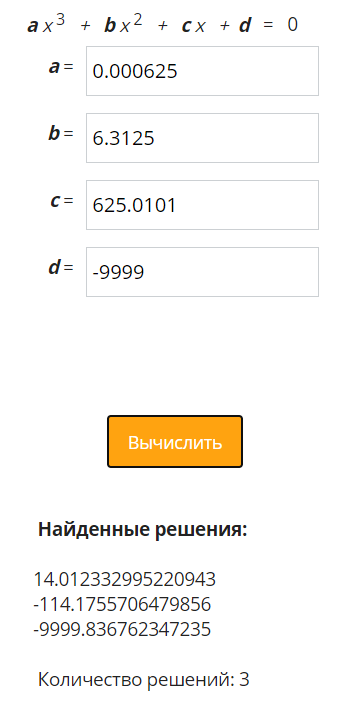
\includegraphics[scale=1]{аналитически.png}
    \caption{Результат вычислений}
\end{figure} 
\newpage
Частота должна быть положительна, поэтому учитываем только первый корень. 
\begin{equation}
    \omega_{кр} = \sqrt{28.0367238} = 5.29497155
\end{equation}
Найдём фазу: 
\begin{equation}
\begin{gathered}
    \phi_{кр}(\omega_{кр}) = -\arctan{T_1\omega_{кр}} -\arctan{T_2\omega_{кр}} -\arctan{T_3\omega_{кр}} = \\
    = -\arctan{132.374288} -\arctan{0.52949} - \arctan{0.052949} = -2.103059
\end{gathered}
\end{equation}
Время запаздывания: 
\begin{equation}
    \tau_{кр} = \frac{\pi - \phi_{кр}}{\omega_{кр}} = 0.195835
\end{equation}
Построим АФЧХ для $\tau < \tau_{кр}, \tau = \tau_{кр}$ и $\tau > \tau_{кр}$ \\
\begin{figure}[h!]
     \centering
    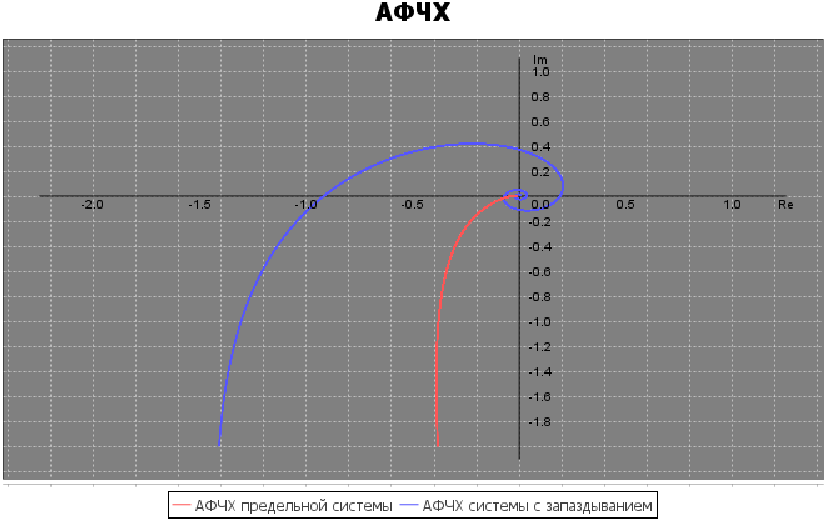
\includegraphics[width = \linewidth]{tau меньше tau крит.png}
    \caption{АФЧХ системы с запаздыванием при $\tau < \tau_{кр}$}
\end{figure} \\
\newpage
\begin{figure}[h!]
     \centering
    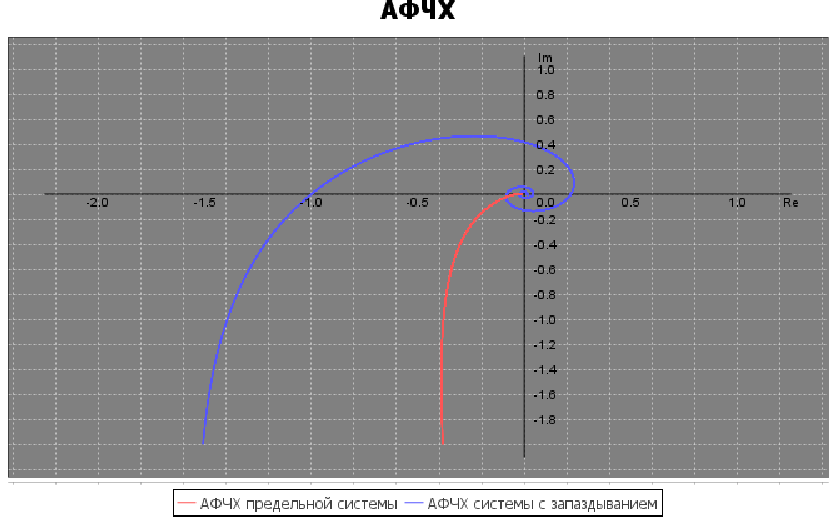
\includegraphics[width = \linewidth]{tau равно tau крит.png}
    \caption{АФЧХ системы с запаздыванием при $\tau = \tau_{кр}$}
\end{figure} 
\begin{figure}[h!]
     \centering
    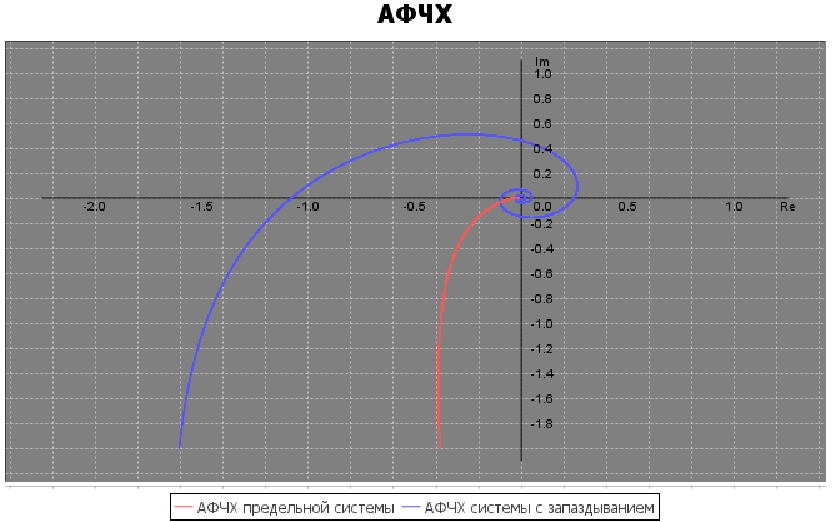
\includegraphics[width = \linewidth]{tau больше tau крит.png}
    \caption{АФЧХ системы с запаздыванием при $\tau > \tau_{кр}$}
\end{figure} 
\newpage
Как видно из графиков, при $\tau < \tau_{кр}$ система устойчива, при $\tau = \tau_{кр}$ система находится на границе устойчивости, а при $\tau > \tau_{кр}$ система неустойчива.
\newpage
\section{Графики переходных функций}
\begin{figure}[h!]
     \centering
    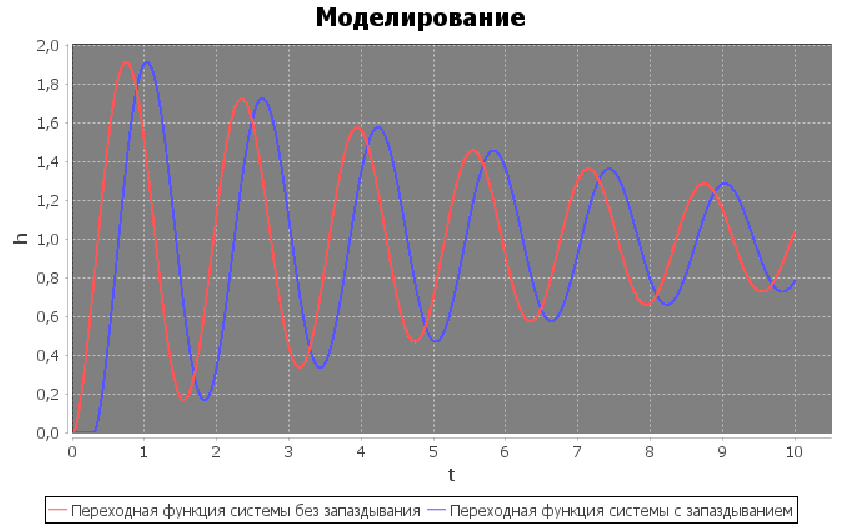
\includegraphics[width = \linewidth]{моделирование 1.png}
    \caption{Моделирование системы при $\tau < \tau_{кр}$}
\end{figure}
\begin{figure}[h!]
     \centering
    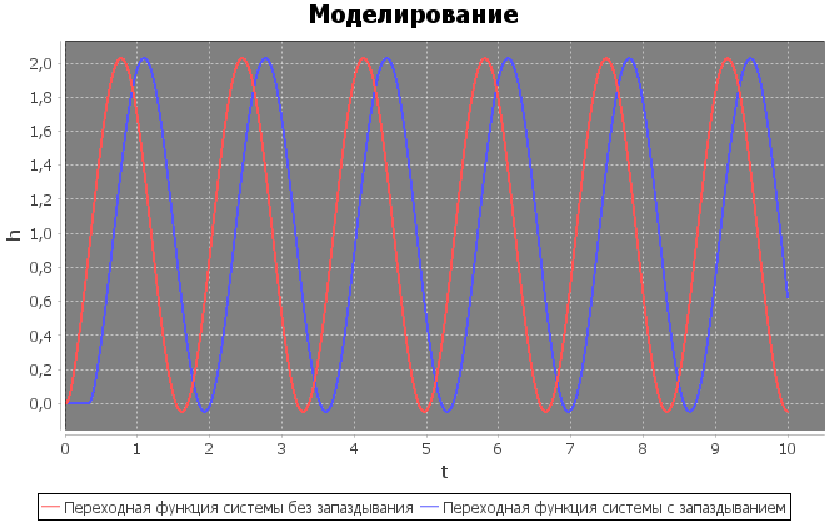
\includegraphics[width = \linewidth]{моделирование 2.png}
    \caption{Моделирование системы при $\tau = \tau_{кр}$}
\end{figure} 
\newpage
\begin{figure}[h!]
     \centering
    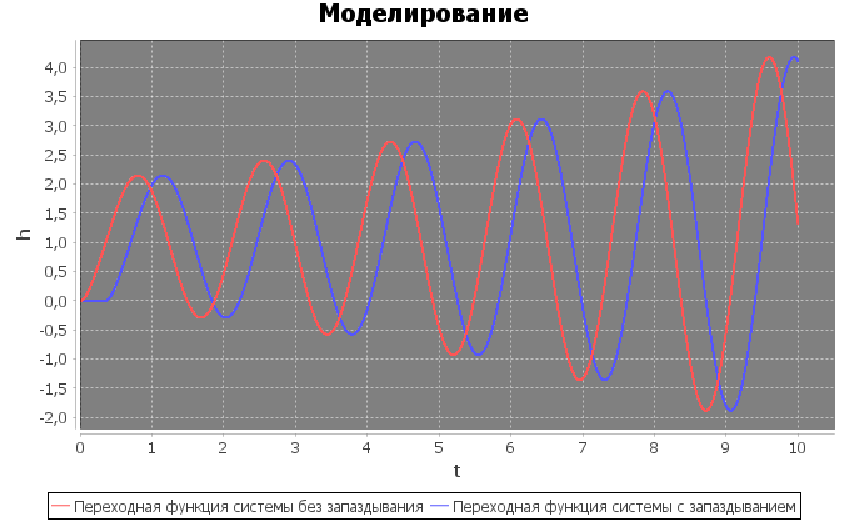
\includegraphics[width = \linewidth]{моделирование 3.png}
    \caption{Моделирование системы при $\tau > \tau_{кр}$}
\end{figure} 
\section{Доказательство правильности определения $\tau_{кр}$}
Из полученных графиков видно, что при $\tau < \tau_{кр}$ переходная функця системы с запаздыванием стремится к 1, значит система находится в устойчивом состоянии; при $\tau = \tau_{кр}$ переходная функция не стремится к какому-либо значению и не расходится, значит система находится на границе устойчивости; при $\tau > \tau_{кр}$ переходная функция расходится, то есть система становится неустойчивой. Эти выводы подтверждают правильность вычисления $\tau_{кр}$. 
\newpage
\section{Влияние запаздывания на качество переходных процессов}
\begin{figure}[h!]
     \centering
    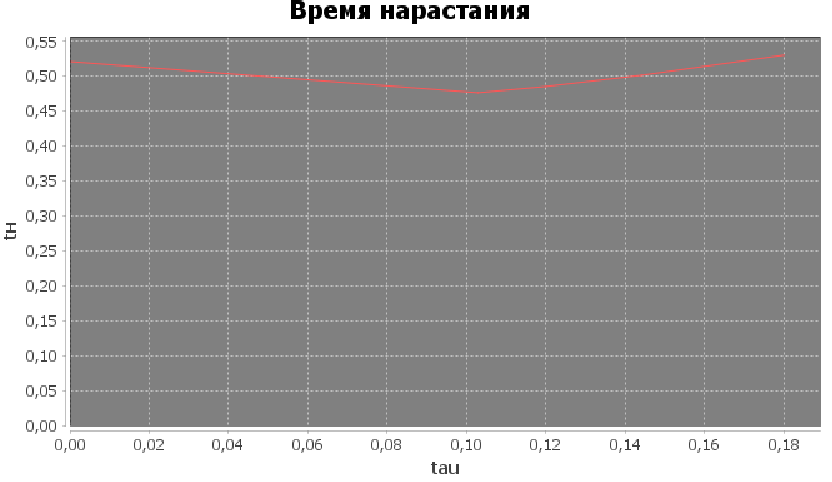
\includegraphics[width = \linewidth]{время нарастания.png}
    \caption{Зависимость времени нарастания от времени запаздывания}
\end{figure} 
\begin{figure}[h!]
     \centering
    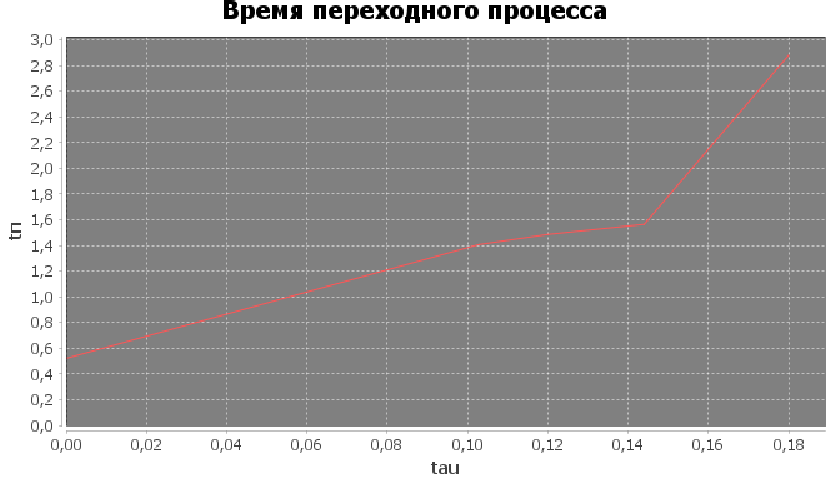
\includegraphics[width = \linewidth]{время переходного процесса.png}
    \caption{Зависимость времени переходного процесса от времени запаздывания}
\end{figure} 
\newpage
\begin{figure}[h!]
     \centering
    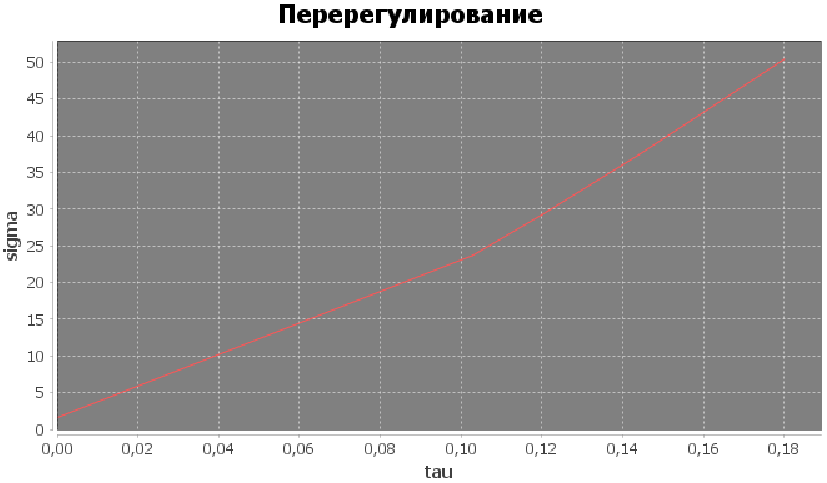
\includegraphics[width = \linewidth]{перерегулирование.png}
    \caption{Зависимость перерегулирования от времени запаздывания}
\end{figure} 
При увеличении времени запаздывания так же увеличиваются и показатели качества, потому что растёт колебательность системы. При дальнейшем увеличении времени запаздывания возникают расходящиея колебания и система становится неустойчивой.  
\newpage
\section{Листинг моделирования}
\lstset{ %
language=Java,                 % выбор языка для подсветки (здесь это С)
basicstyle=\small\sffamily, % размер и начертание шрифта для подсветки кода
numbers=left,               % где поставить нумерацию строк (слева\справа)
numberstyle=\tiny,           % размер шрифта для номеров строк
stepnumber=1,                   % размер шага между двумя номерами строк
numbersep=5pt,                % как далеко отстоят номера строк от подсвечиваемого кода
backgroundcolor=\color{white}, % цвет фона подсветки - используем \usepackage{color}
showspaces=false,            % показывать или нет пробелы специальными отступами
showstringspaces=false,      % показывать или нет пробелы в строках
showtabs=false,             % показывать или нет табуляцию в строках
frame=single,              % рисовать рамку вокруг кода
tabsize=2,                 % размер табуляции по умолчанию равен 2 пробелам
captionpos=t,              % позиция заголовка вверху [t] или внизу [b] 
breaklines=true,           % автоматически переносить строки (да\нет)
breakatwhitespace=false, % переносить строки только если есть пробел
escapeinside={\%*}{*)}   % если нужно добавить комментарии в коде
}
\begin{lstlisting}
      public void addGraph(String title, double tau) {
       double std = 0, x, g=1, y=0, y1=0, y2=0, y3=0;
        int ns = (int) (tau/dt), i=0;
        VectorSeries y_ser = new VectorSeries("Transitional function");
        VectorSeries delay_ser = new VectorSeries(title);
        while(std < l) {
            x = g - y;

            y1 += getY(1/T1, k/T1, x, y1);
            y2 += getY(1/T2, 1/T2, y1, y2);
            y3 += getY(1/T3, 1/T3, y2, y3);

            y_ser.add(std, y3, 0, 0);

            if(i > ns) {
                y = y_ser.getYValue(i - ns);
            }
            else
                y = 0;
            i++;
            delay_ser.add(std, y, 0, 0);

            std += dt;
        }
        collection.addSeries(y_ser);
        collection.addSeries(delay_ser);
    }
    private double getY(double a0, double alpha, double x, double z) {
        double K1, K2, K3, K4;
        K1 = (-a0*z + alpha*x)*dt;
        K2 = (-a0*(z + K1/2) + alpha*x)*dt;
        K3 = (-a0*(z + K2/2) + alpha*x)*dt;
        K4 = (-a0*(z + K3) + alpha*x)*dt;
        return (K1 + 2*K2 + 2*K3 + K4)/6;
    }
\end{lstlisting}
\newpage
\end{document}
